\usection{Lecture 10: Dynamic games (cont.)}
\newsection
\subsection*{Recap}
\begin{enumerate}
    \item Dynamic (Multi-stage) games.
    \item Game tree (extensive form game)
    \item Sequential rationality - subgame-perfect Nash equilibrium using backward induction.
\end{enumerate}

\begin{aexample}{3 period Bargaining}{}
    Two players are splitting one dollar. 
    They follow an alternating offer bargaining model. The game is terminated when one player accepts.
    
    \begin{itemize}
        \item Period 1: Player 1 makes an offer $(s_1,1-s_1)$. Player 2 can accept or reject the offer.
        \item Period 2: Player 2 makes an offer $(s_2,1-s_2)$. Player 1 can accept or reject.
        \item Period 3: The players get $(s,1-s)$.
    \end{itemize}

    Let $\delta\in(0,1)$. This is the discounted payoff, i.e. how much they discount the future payoff. Therefore, we rewrite it as:
    \begin{itemize}
        \item [1:] Player 1 makes an offer $(s_1,1-s_1)$. Player 2 can accept or reject the offer.
        \item [2:] Player 2 makes an offer $(\delta s_2,\delta(1-s_2))$. Player 1 can accept or reject.
        \item [3:] The players get $(\delta^2 s,\delta^2(1-s))$.
    \end{itemize}
    Work out the SPNE of the game.
\end{aexample}
Using backward induction, for period 2, player 1's response is \[
\begin{cases}
    \rm{accept,} & \textrm{if }\delta s_2\geq \delta^2s\implies s_2\geq \delta s,\\
    \rm{reject,} & \textrm{otherwise.} 
\end{cases}
\]
So player 2 can offer $(\delta s, 1-\delta s)$ with an intention to get $\delta (1-\delta s)$.
Therefore, player 2 rejects player 1's offer in period 1 if \[
1-s_1<\delta (1-\delta s)
\]
Player 1 thus makes, in period 1, an offer of \[
s_1= 1-\delta(1-\delta s)=(1-\delta) + \delta^2 s.
\]

There is an extension of this model. 

\begin{aexample}{Infinite horizon alternate bargaining}{}
    Two players are splitting one dollar. 
    Let $\delta\in(0,1)$. Therefore, we rewrite it as:
    \begin{itemize}
        \item [1:] Player 1 makes an offer $(s_1,1-s_1)$. Player 2 can accept or reject the offer.
        \item [2:] Player 2 makes an offer $(s_2,(1-s_2))$. Player 1 can accept or reject.
        \item [3:] return to period 1. 
    \end{itemize}
    Work out the SPNE of the game.
\end{aexample}

There is no way to use backward induction of the game. However, there is a (cheesy) recursive way. Notice at period 3 onwards, the game is identical to the game starting at period one with splitting a $\delta^2$ dollar bill. 

Now suppose that there is an SPNE in period 3 that gives a payoff $(a,b)$, then period 1 player 1 can get a payoff of \[
1-\delta(1-\delta a)=a \implies a=\frac{1}{1+\delta}.
\]

\begin{aexample}{Centipede}{}
    Consider:
    \begin{center}
    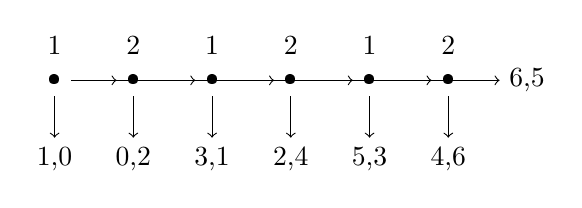
\begin{tikzpicture}
        \node [label={above: 1}] (A) at (0,0) {\textbullet};
        \node (AA) at(0,-1) {1,0};
        \node[label={above: 2}] (B)at (1,0) {\textbullet};
        \node (BB)  at (1,-1) {0,2};
        \node[label={above: 1}] (C)at (2,0) {\textbullet};
        \node (CC) at (2,-1) {3,1};
        \node[label={above: 2}] (D)at (3,0) {\textbullet};
        \node (DD)at (3,-1) {2,4};
        \node[label={above: 1}] (E)at (4,0) {\textbullet};
        \node(EE) at (4,-1) {5,3};
        \node[label={above: 2}] (F)at (5,0) {\textbullet};
        \node (FF)at (5,-1) {4,6};
        \node (G)at (6,0) {6,5};
        
            \draw[->] (A)edge (B)edge (C)edge (D)edge (E)edge (F)edge (G);\draw[->](A) edge(AA);
            \draw[->](B) edge(BB);
            \draw[->](C) edge(CC);
            \draw[->](D) edge(DD);
            \draw[->](E) edge(EE);
            \draw[->](F) edge(FF);

    \end{tikzpicture}
\end{center}
    Intuitively, the sequence should continue sometime into the right. However, the SPNE actually results in (1,0)!
\end{aexample}
Or \begin{center}
    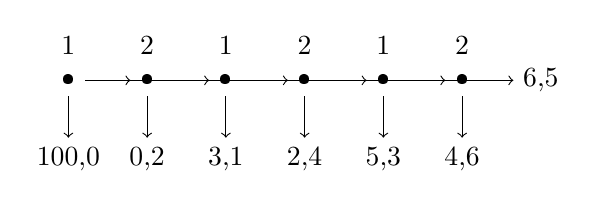
\begin{tikzpicture}
        \node [label={above: 1}] (A) at (0,0) {\textbullet};
        \node (AA) at(0,-1) {100,0};
        \node[label={above: 2}] (B)at (1,0) {\textbullet};
        \node (BB)  at (1,-1) {0,2};
        \node[label={above: 1}] (C)at (2,0) {\textbullet};
        \node (CC) at (2,-1) {3,1};
        \node[label={above: 2}] (D)at (3,0) {\textbullet};
        \node (DD)at (3,-1) {2,4};
        \node[label={above: 1}] (E)at (4,0) {\textbullet};
        \node(EE) at (4,-1) {5,3};
        \node[label={above: 2}] (F)at (5,0) {\textbullet};
        \node (FF)at (5,-1) {4,6};
        \node (G)at (6,0) {6,5};
        
            \draw[->] (A)edge (B)edge (C)edge (D)edge (E)edge (F)edge (G);\draw[->](A) edge(AA);
            \draw[->](B) edge(BB);
            \draw[->](C) edge(CC);
            \draw[->](D) edge(DD);
            \draw[->](E) edge(EE);
            \draw[->](F) edge(FF);

    \end{tikzpicture}
\end{center}
In this case, we do not even consider what player 1 would do in the right, because the first choice dominates all possiblities. It is not certain that people think of subgames.


\definition{Information set}{
    An information set is a collection of decision nodes that are indistinguishable for the player making the decision at the nodes.
}

We can also adjust the extensive form representation by drawing a circle/dashed line across indistinguishable subgames.
\begin{center}
    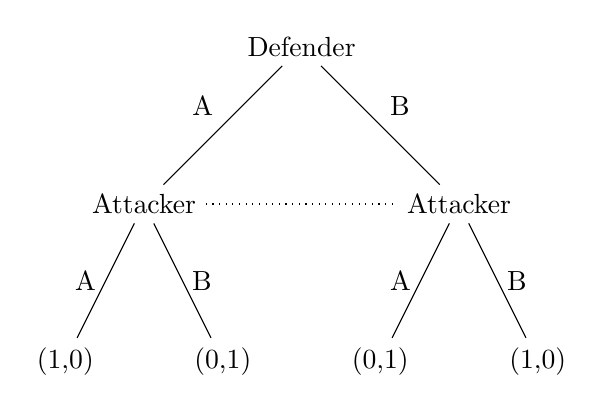
\begin{tikzpicture}
        \node (A) at (0,0){Defender};
        \node(B) at (-2,-2) {Attacker};
        \node(C) at (2,-2) {Attacker};
        \node(D) at (-3,-4) {(1,0)};
        \node(E) at (-1,-4) {(0,1)};
        \node(F) at (1,-4) {(0,1)};
        \node(G) at (3,-4) {(1,0)};
        \draw (A) edge  node[midway, above left]{A}(B);
        \draw (A) edge  node[midway, above right]{B}(C);
        \draw (B) edge  node[midway,  left]{A}(D);
        \draw (B) edge node[midway,  right]{B} (E) ;
        \draw (C) edge  node[midway,  left]{A}(F);
        \draw (C) edge  node[midway,  right]{B}(G);
        \draw [dotted] (B)edge (C);
    \end{tikzpicture}\end{center}

    In this case, the Attacker cannot distinguish the subgames depending on what the Defender picked. The defender's information set is a singleton. 
    \definition{Perfect information game}{
        If every information set is a singleton, we call the game a \textbf{game with perfect information.}
    }

\begin{aexample}{}{}
    
\begin{center}
    \begin{tikzpicture}
        \node(a) at (-2,4){1};
        \node(b) at (-3,2){(2,2)};
        \node(c) at (-1,2){2};
        \node(d) at (-2,0){(1,2)};
        \draw (a) edge  node[midway, above left]{L}(b);\draw (a) edge  node[midway, above right]{R}(c);
        \draw (c) edge node[midway, above left]{L} (d);
        \draw (c) edge node[midway, above right]{R} (A);

        \node (A) at (0,0){1};
        \node(B) at (-2,-2) {2};
        \node(C) at (2,-2) {2};
        \node(D) at (-3,-4) {(2,5)};
        \node(E) at (-1,-4) {(0,0)};
        \node(F) at (1,-4) {(3,0)};
        \node(G) at (3,-4) {(1,1)};
        \draw (A) edge  node[midway, above left]{A}(B);
        \draw (A) edge  node[midway, above right]{B}(C);
        \draw (B) edge  node[midway,  left]{C}(D);
        \draw (B) edge node[midway,  right]{D} (E) ;
        \draw (C) edge  node[midway,  left]{C}(F);
        \draw (C) edge  node[midway,  right]{D}(G);
        \draw [dotted] (B)edge (C);
    \end{tikzpicture}\end{center}
\end{aexample}
We need to work on \textbf{proper subgames}, games that start at a singleton and does not break any information set. 
Starting with the second decision tree of 1, 
payoff matrix of \begin{center}
    \begin{tabular}{|c c|}
            \hline (2,5) & (0,0)\\ \hline (3,0) & (1,1)\\ \hline
    \end{tabular}
\end{center}
has a Nash equilibrium of (B,D). Then 2 chooses between (1,2) and (1,1), so would decide L in the tree. Finally 1's first decision between (2,2) and (1,2) will lead to a SPNE result of (2,2).

\begin{aexample}{Bank Runs}{}
    There are two investors. Each puts $D$ dollars in the bank. This money is invested in a long term project.
    
    \begin{itemize}
        \item Period 1: The investors can withdraw or stay invested. Pulling out now will get a return of $2r$, $r\in (D,D/2)$.
        \item Period 2: If investment matures, the return is $2R$, $R>D$.
    \end{itemize}
    \begin{center}
    \begin{tabular}{|c|c c|}
        \hline period 1& W & S\\
            \hline  W & (r,r) & (D,2r-D)\\ \hline S& (2r-D,D) & next stage\\ \hline
    \end{tabular}
\end{center}
\begin{center}
    \begin{tabular}{|c|c c|}
        \hline period 2 & W & S\\
            \hline  W & (R,R) & (D,2R-D)\\ \hline S& (2R-D,D) & (R,R)\\ \hline
    \end{tabular}
\end{center}
\end{aexample}
Putting (R,R) into the next stage, there are two nash equilibria (r,r) and (R,R).

\begin{aexample}{Investment and Price Competition}{}
    2 Firms first decide to invest and enter a new market at a cost of $c_i$. If both enter, they compete on price (Betrand competition). If one enters, they get to be a monopolist. If no one enters, the payoffs are zero.
\end{aexample}

   
\begin{center}
    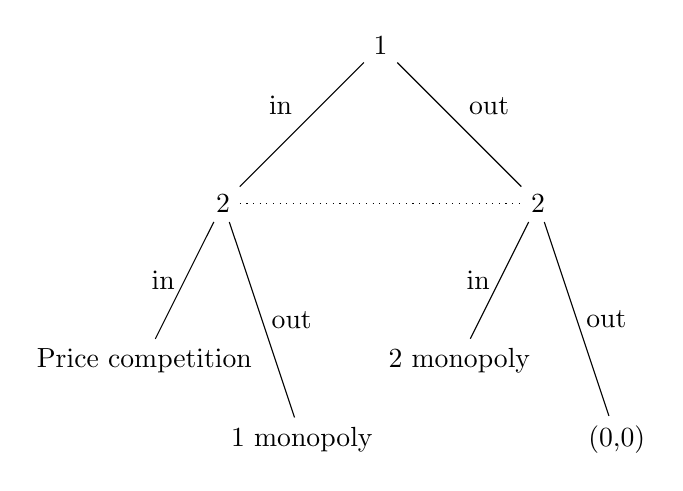
\begin{tikzpicture}
        \node (A) at (0,0){1};
        \node(B) at (-2,-2) {2};
        \node(C) at (2,-2) {2};
        \node(D) at (-3,-4) {Price competition};
        \node(E) at (-1,-5) {1 monopoly};
        \node(F) at (1,-4) {2 monopoly};
        \node(G) at (3,-5) {(0,0)};
        \draw (A) edge  node[midway, above left]{in}(B);
        \draw (A) edge  node[midway, above right]{out}(C);
        \draw (B) edge  node[midway,  left]{in}(D);
        \draw (B) edge node[midway,  right]{out} (E) ;
        \draw (C) edge  node[midway,  left]{in}(F);
        \draw (C) edge  node[midway,  right]{out}(G);
        \draw [dotted] (B)edge (C);
    \end{tikzpicture}\end{center}
    The price competition results in a payoff of $(-c_1,-c_2)$. The monopolist gains $(1/4-c_i)$.
    We therefore have a payoff matrix in the first round:
    \begin{center}
        \begin{tabular}{|c|c c|}
            \hline period 1& in & out\\
                \hline  in & $(-c_1,-c_2)$ & $(1/4-c_1,0)$\\ \hline out& $(0,1/4-c_2)$ & $(0,0)$\\ \hline
        \end{tabular}
    \end{center}
    If both $c_1,c_2>1/4$, then both will want to withdraw the market. If both of them are smaller, the nash equilibrium is that one of the firms enter the market as a Nash equilibrium. If exactly one of them has $c_i\leq 1/4$, then that firm enters the market.

    